\documentclass[1p]{elsarticle_modified}
%\bibliographystyle{elsarticle-num}

%\usepackage[colorlinks]{hyperref}
%\usepackage{abbrmath_seonhwa} %\Abb, \Ascr, \Acal ,\Abf, \Afrak
\usepackage{amsfonts}
\usepackage{amssymb}
\usepackage{amsmath}
\usepackage{amsthm}
\usepackage{scalefnt}
\usepackage{amsbsy}
\usepackage{kotex}
\usepackage{caption}
\usepackage{subfig}
\usepackage{color}
\usepackage{graphicx}
\usepackage{xcolor} %% white, black, red, green, blue, cyan, magenta, yellow
\usepackage{float}
\usepackage{setspace}
\usepackage{hyperref}

\usepackage{tikz}
\usetikzlibrary{arrows}

\usepackage{multirow}
\usepackage{array} % fixed length table
\usepackage{hhline}

%%%%%%%%%%%%%%%%%%%%%
\makeatletter
\renewcommand*\env@matrix[1][\arraystretch]{%
	\edef\arraystretch{#1}%
	\hskip -\arraycolsep
	\let\@ifnextchar\new@ifnextchar
	\array{*\c@MaxMatrixCols c}}
\makeatother %https://tex.stackexchange.com/questions/14071/how-can-i-increase-the-line-spacing-in-a-matrix
%%%%%%%%%%%%%%%

\usepackage[normalem]{ulem}

\newcommand{\msout}[1]{\ifmmode\text{\sout{\ensuremath{#1}}}\else\sout{#1}\fi}
%SOURCE: \msout is \stkout macro in https://tex.stackexchange.com/questions/20609/strikeout-in-math-mode

\newcommand{\cancel}[1]{
	\ifmmode
	{\color{red}\msout{#1}}
	\else
	{\color{red}\sout{#1}}
	\fi
}

\newcommand{\add}[1]{
	{\color{blue}\uwave{#1}}
}

\newcommand{\replace}[2]{
	\ifmmode
	{\color{red}\msout{#1}}{\color{blue}\uwave{#2}}
	\else
	{\color{red}\sout{#1}}{\color{blue}\uwave{#2}}
	\fi
}

\newcommand{\Sol}{\mathcal{S}} %segment
\newcommand{\D}{D} %diagram
\newcommand{\A}{\mathcal{A}} %arc


%%%%%%%%%%%%%%%%%%%%%%%%%%%%%5 test

\def\sl{\operatorname{\textup{SL}}(2,\Cbb)}
\def\psl{\operatorname{\textup{PSL}}(2,\Cbb)}
\def\quan{\mkern 1mu \triangleright \mkern 1mu}

\theoremstyle{definition}
\newtheorem{thm}{Theorem}[section]
\newtheorem{prop}[thm]{Proposition}
\newtheorem{lem}[thm]{Lemma}
\newtheorem{ques}[thm]{Question}
\newtheorem{cor}[thm]{Corollary}
\newtheorem{defn}[thm]{Definition}
\newtheorem{exam}[thm]{Example}
\newtheorem{rmk}[thm]{Remark}
\newtheorem{alg}[thm]{Algorithm}

\newcommand{\I}{\sqrt{-1}}
\begin{document}

%\begin{frontmatter}
%
%\title{Boundary parabolic representations of knots up to 8 crossings}
%
%%% Group authors per affiliation:
%\author{Yunhi Cho} 
%\address{Department of Mathematics, University of Seoul, Seoul, Korea}
%\ead{yhcho@uos.ac.kr}
%
%
%\author{Seonhwa Kim} %\fnref{s_kim}}
%\address{Center for Geometry and Physics, Institute for Basic Science, Pohang, 37673, Korea}
%\ead{ryeona17@ibs.re.kr}
%
%\author{Hyuk Kim}
%\address{Department of Mathematical Sciences, Seoul National University, Seoul 08826, Korea}
%\ead{hyukkim@snu.ac.kr}
%
%\author{Seokbeom Yoon}
%\address{Department of Mathematical Sciences, Seoul National University, Seoul, 08826,  Korea}
%\ead{sbyoon15@snu.ac.kr}
%
%\begin{abstract}
%We find all boundary parabolic representation of knots up to 8 crossings.
%
%\end{abstract}
%\begin{keyword}
%    \MSC[2010] 57M25 
%\end{keyword}
%
%\end{frontmatter}

%\linenumbers
%\tableofcontents
%
\newcommand\colored[1]{\textcolor{white}{\rule[-0.35ex]{0.8em}{1.4ex}}\kern-0.8em\color{red} #1}%
%\newcommand\colored[1]{\textcolor{white}{ #1}\kern-2.17ex	\textcolor{white}{ #1}\kern-1.81ex	\textcolor{white}{ #1}\kern-2.15ex\color{red}#1	}

{\Large $\underline{12a_{0545}~(K12a_{0545})}$}

\setlength{\tabcolsep}{10pt}
\renewcommand{\arraystretch}{1.6}
\vspace{1cm}\begin{tabular}{m{100pt}>{\centering\arraybackslash}m{274pt}}
\multirow{5}{120pt}{
	\centering
	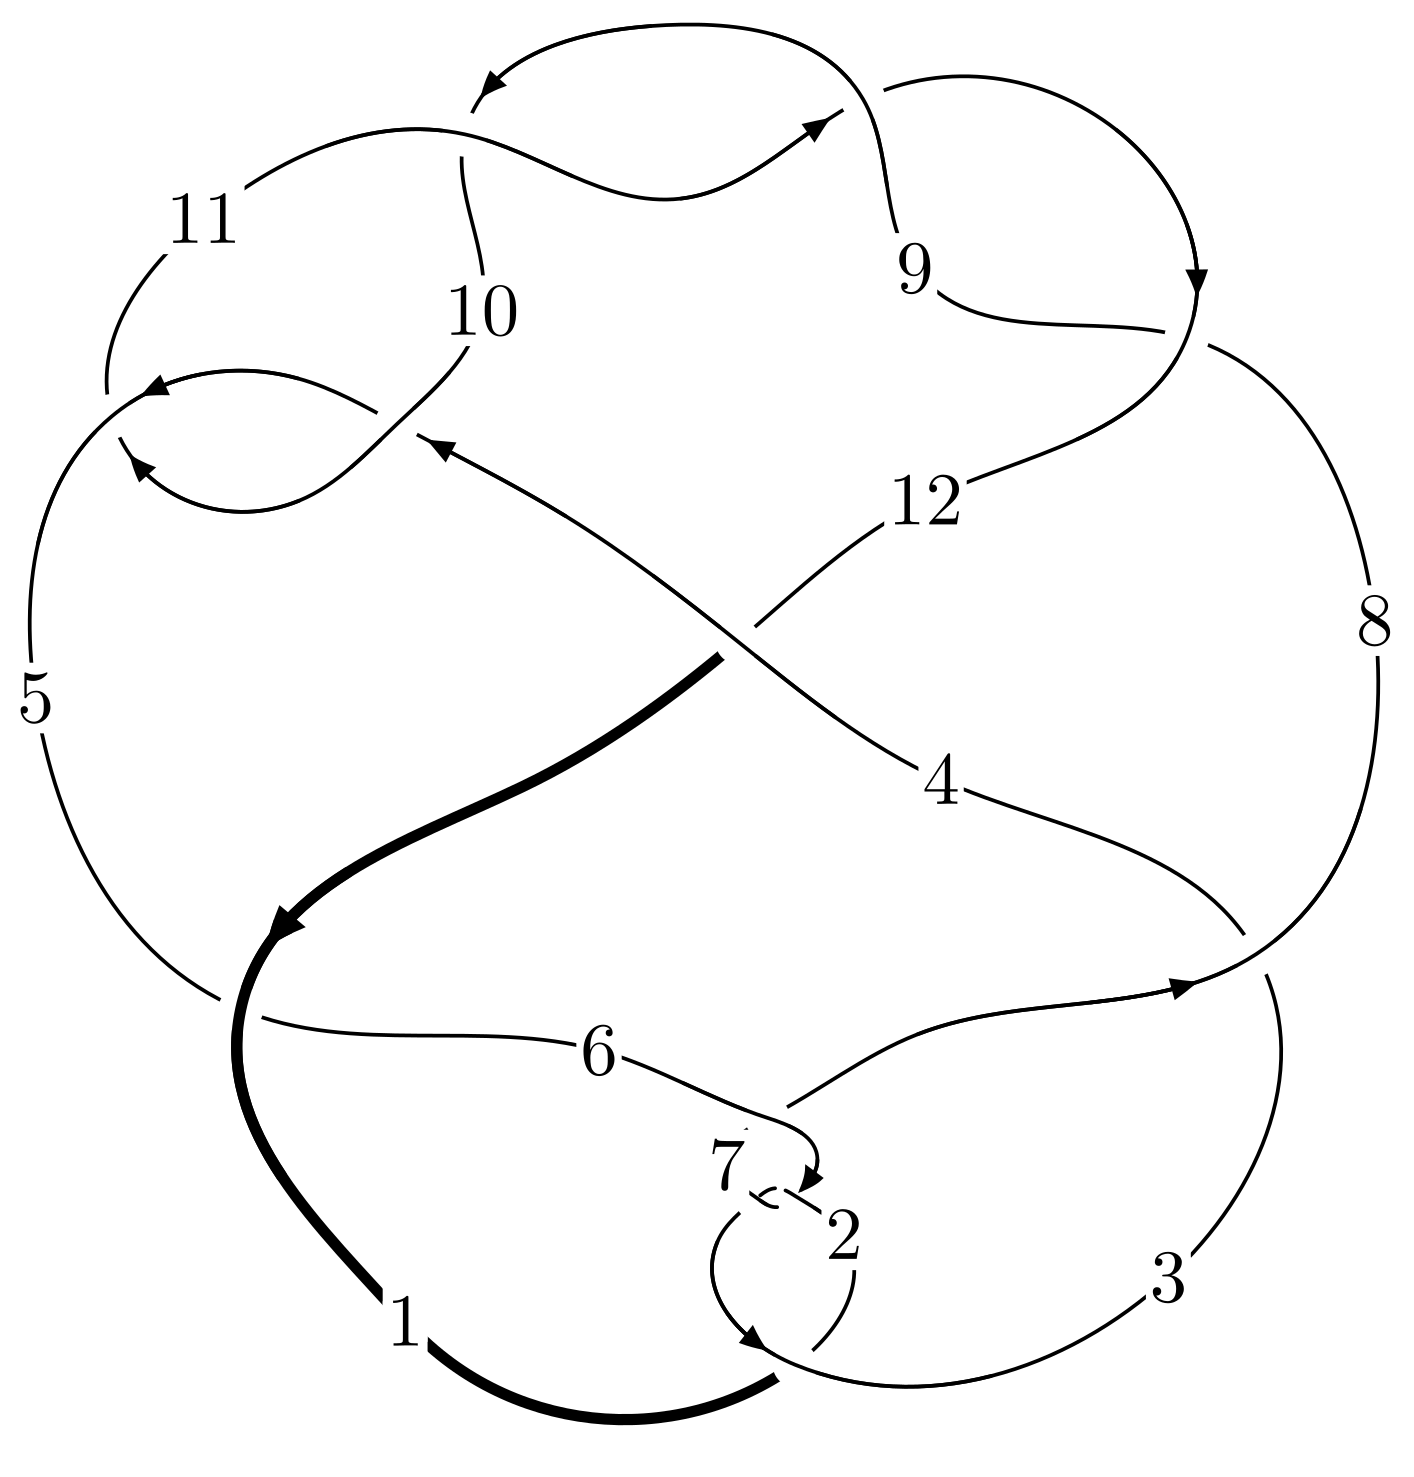
\includegraphics[width=112pt]{../../../GIT/diagram.site/Diagrams/png/1346_12a_0545.png}\\
\ \ \ A knot diagram\footnotemark}&
\allowdisplaybreaks
\textbf{Linearized knot diagam} \\
\cline{2-2}
 &
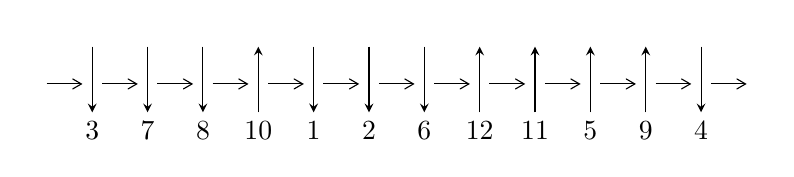
\begin{tikzpicture}[x=20pt, y=17pt]
	% nodes
	\node (C0) at (0, 0) {};
	\node (C1) at (1, 0) {};
	\node (C1U) at (1, +1) {};
	\node (C1D) at (1, -1) {3};

	\node (C2) at (2, 0) {};
	\node (C2U) at (2, +1) {};
	\node (C2D) at (2, -1) {7};

	\node (C3) at (3, 0) {};
	\node (C3U) at (3, +1) {};
	\node (C3D) at (3, -1) {8};

	\node (C4) at (4, 0) {};
	\node (C4U) at (4, +1) {};
	\node (C4D) at (4, -1) {10};

	\node (C5) at (5, 0) {};
	\node (C5U) at (5, +1) {};
	\node (C5D) at (5, -1) {1};

	\node (C6) at (6, 0) {};
	\node (C6U) at (6, +1) {};
	\node (C6D) at (6, -1) {2};

	\node (C7) at (7, 0) {};
	\node (C7U) at (7, +1) {};
	\node (C7D) at (7, -1) {6};

	\node (C8) at (8, 0) {};
	\node (C8U) at (8, +1) {};
	\node (C8D) at (8, -1) {12};

	\node (C9) at (9, 0) {};
	\node (C9U) at (9, +1) {};
	\node (C9D) at (9, -1) {11};

	\node (C10) at (10, 0) {};
	\node (C10U) at (10, +1) {};
	\node (C10D) at (10, -1) {5};

	\node (C11) at (11, 0) {};
	\node (C11U) at (11, +1) {};
	\node (C11D) at (11, -1) {9};

	\node (C12) at (12, 0) {};
	\node (C12U) at (12, +1) {};
	\node (C12D) at (12, -1) {4};
	\node (C13) at (13, 0) {};

	% arrows
	\draw[->,>={angle 60}]
	(C0) edge (C1) (C1) edge (C2) (C2) edge (C3) (C3) edge (C4) (C4) edge (C5) (C5) edge (C6) (C6) edge (C7) (C7) edge (C8) (C8) edge (C9) (C9) edge (C10) (C10) edge (C11) (C11) edge (C12) (C12) edge (C13) ;	\draw[->,>=stealth]
	(C1U) edge (C1D) (C2U) edge (C2D) (C3U) edge (C3D) (C4D) edge (C4U) (C5U) edge (C5D) (C6U) edge (C6D) (C7U) edge (C7D) (C8D) edge (C8U) (C9D) edge (C9U) (C10D) edge (C10U) (C11D) edge (C11U) (C12U) edge (C12D) ;
	\end{tikzpicture} \\
\hhline{~~} \\& 
\textbf{Solving Sequence} \\ \cline{2-2} 
 &
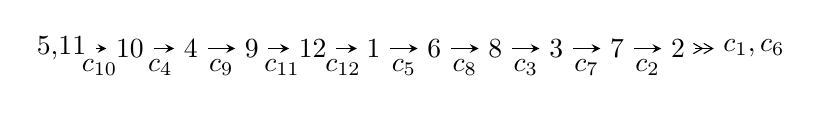
\begin{tikzpicture}[x=22pt, y=7pt]
	% node
	\node (A0) at (-1/8, 0) {5,11};
	\node (A1) at (1, 0) {10};
	\node (A2) at (2, 0) {4};
	\node (A3) at (3, 0) {9};
	\node (A4) at (4, 0) {12};
	\node (A5) at (5, 0) {1};
	\node (A6) at (6, 0) {6};
	\node (A7) at (7, 0) {8};
	\node (A8) at (8, 0) {3};
	\node (A9) at (9, 0) {7};
	\node (A10) at (10, 0) {2};
	\node (C1) at (1/2, -1) {$c_{10}$};
	\node (C2) at (3/2, -1) {$c_{4}$};
	\node (C3) at (5/2, -1) {$c_{9}$};
	\node (C4) at (7/2, -1) {$c_{11}$};
	\node (C5) at (9/2, -1) {$c_{12}$};
	\node (C6) at (11/2, -1) {$c_{5}$};
	\node (C7) at (13/2, -1) {$c_{8}$};
	\node (C8) at (15/2, -1) {$c_{3}$};
	\node (C9) at (17/2, -1) {$c_{7}$};
	\node (C10) at (19/2, -1) {$c_{2}$};
	\node (A11) at (45/4, 0) {$c_{1},c_{6}$};

	% edge
	\draw[->,>=stealth]	
	(A0) edge (A1) (A1) edge (A2) (A2) edge (A3) (A3) edge (A4) (A4) edge (A5) (A5) edge (A6) (A6) edge (A7) (A7) edge (A8) (A8) edge (A9) (A9) edge (A10) ;
	\draw[->>,>={angle 60}]	
	(A10) edge (A11);
\end{tikzpicture} \\ 

\end{tabular} \\

\footnotetext{
The image of knot diagram is generated by the software ``\textbf{Draw programme}" developed by Andrew Bartholomew(\url{http://www.layer8.co.uk/maths/draw/index.htm\#Running-draw}), where we modified some parts for our purpose(\url{https://github.com/CATsTAILs/LinksPainter}).
}\phantom \\ \newline 
\centering \textbf{Ideals for irreducible components\footnotemark of $X_{\text{par}}$} 
 
\begin{align*}
I^u_{1}&=\langle 
u^{71}- u^{70}+\cdots+2 u-1\rangle \\
\\
\end{align*}
\raggedright * 1 irreducible components of $\dim_{\mathbb{C}}=0$, with total 71 representations.\\
\footnotetext{All coefficients of polynomials are rational numbers. But the coefficients are sometimes approximated in decimal forms when there is not enough margin.}
\newpage
\renewcommand{\arraystretch}{1}
\centering \section*{I. $I^u_{1}= \langle u^{71}- u^{70}+\cdots+2 u-1 \rangle$}
\flushleft \textbf{(i) Arc colorings}\\
\begin{tabular}{m{7pt} m{180pt} m{7pt} m{180pt} }
\flushright $a_{5}=$&$\begin{pmatrix}0\\u\end{pmatrix}$ \\
\flushright $a_{11}=$&$\begin{pmatrix}1\\0\end{pmatrix}$ \\
\flushright $a_{10}=$&$\begin{pmatrix}1\\u^2\end{pmatrix}$ \\
\flushright $a_{4}=$&$\begin{pmatrix}- u\\- u^3+u\end{pmatrix}$ \\
\flushright $a_{9}=$&$\begin{pmatrix}- u^2+1\\u^2\end{pmatrix}$ \\
\flushright $a_{12}=$&$\begin{pmatrix}u^4- u^2+1\\- u^4\end{pmatrix}$ \\
\flushright $a_{1}=$&$\begin{pmatrix}u^8- u^6+3 u^4-2 u^2+1\\u^{10}-2 u^8+3 u^6-4 u^4+u^2\end{pmatrix}$ \\
\flushright $a_{6}=$&$\begin{pmatrix}- u^{17}+2 u^{15}-7 u^{13}+10 u^{11}-15 u^9+14 u^7-10 u^5+4 u^3- u\\- u^{19}+3 u^{17}-8 u^{15}+15 u^{13}-19 u^{11}+21 u^9-14 u^7+6 u^5- u^3+u\end{pmatrix}$ \\
\flushright $a_{8}=$&$\begin{pmatrix}- u^6+u^4-2 u^2+1\\u^6+u^2\end{pmatrix}$ \\
\flushright $a_{3}=$&$\begin{pmatrix}- u^{15}+2 u^{13}-6 u^{11}+8 u^9-10 u^7+8 u^5-4 u^3\\u^{15}- u^{13}+4 u^{11}-3 u^9+4 u^7-2 u^5+u\end{pmatrix}$ \\
\flushright $a_{7}=$&$\begin{pmatrix}u^{42}-5 u^{40}+\cdots- u^2+1\\u^{44}-6 u^{42}+\cdots-12 u^6+3 u^4\end{pmatrix}$ \\
\flushright $a_{2}=$&$\begin{pmatrix}- u^{40}+5 u^{38}+\cdots-2 u^2+1\\u^{40}-4 u^{38}+\cdots-6 u^4+2 u^2\end{pmatrix}$\\&\end{tabular}
\flushleft \textbf{(ii) Obstruction class $= -1$}\\~\\
\flushleft \textbf{(iii) Cusp Shapes $= 4 u^{69}-4 u^{68}+\cdots-8 u-6$}\\~\\
\newpage\renewcommand{\arraystretch}{1}
\flushleft \textbf{(iv) u-Polynomials at the component}\newline \\
\begin{tabular}{m{50pt}|m{274pt}}
Crossings & \hspace{64pt}u-Polynomials at each crossing \\
\hline $$\begin{aligned}c_{1},c_{7}\end{aligned}$$&$\begin{aligned}
&u^{71}+25 u^{70}+\cdots+4 u+1
\end{aligned}$\\
\hline $$\begin{aligned}c_{2},c_{6}\end{aligned}$$&$\begin{aligned}
&u^{71}- u^{70}+\cdots-2 u+1
\end{aligned}$\\
\hline $$\begin{aligned}c_{3},c_{5}\end{aligned}$$&$\begin{aligned}
&u^{71}+u^{70}+\cdots-406 u+97
\end{aligned}$\\
\hline $$\begin{aligned}c_{4},c_{10}\end{aligned}$$&$\begin{aligned}
&u^{71}+u^{70}+\cdots+2 u+1
\end{aligned}$\\
\hline $$\begin{aligned}c_{8},c_{9},c_{11}\end{aligned}$$&$\begin{aligned}
&u^{71}-17 u^{70}+\cdots+4 u-1
\end{aligned}$\\
\hline $$\begin{aligned}c_{12}\end{aligned}$$&$\begin{aligned}
&u^{71}-7 u^{70}+\cdots+13008 u-6545
\end{aligned}$\\
\hline
\end{tabular}\\~\\
\newpage\renewcommand{\arraystretch}{1}
\flushleft \textbf{(v) Riley Polynomials at the component}\newline \\
\begin{tabular}{m{50pt}|m{274pt}}
Crossings & \hspace{64pt}Riley Polynomials at each crossing \\
\hline $$\begin{aligned}c_{1},c_{7}\end{aligned}$$&$\begin{aligned}
&y^{71}+43 y^{70}+\cdots-20 y-1
\end{aligned}$\\
\hline $$\begin{aligned}c_{2},c_{6}\end{aligned}$$&$\begin{aligned}
&y^{71}-25 y^{70}+\cdots+4 y-1
\end{aligned}$\\
\hline $$\begin{aligned}c_{3},c_{5}\end{aligned}$$&$\begin{aligned}
&y^{71}-53 y^{70}+\cdots+348748 y-9409
\end{aligned}$\\
\hline $$\begin{aligned}c_{4},c_{10}\end{aligned}$$&$\begin{aligned}
&y^{71}-17 y^{70}+\cdots+4 y-1
\end{aligned}$\\
\hline $$\begin{aligned}c_{8},c_{9},c_{11}\end{aligned}$$&$\begin{aligned}
&y^{71}+75 y^{70}+\cdots-20 y-1
\end{aligned}$\\
\hline $$\begin{aligned}c_{12}\end{aligned}$$&$\begin{aligned}
&y^{71}-25 y^{70}+\cdots+292384964 y-42837025
\end{aligned}$\\
\hline
\end{tabular}\\~\\
\newpage\flushleft \textbf{(vi) Complex Volumes and Cusp Shapes}
$$\begin{array}{c|c|c}  
\text{Solutions to }I^u_{1}& \I (\text{vol} + \sqrt{-1}CS) & \text{Cusp shape}\\
 \hline 
\begin{aligned}
u &= -0.888190 + 0.459117 I\end{aligned}
 & -1.18643 + 1.35824 I & \phantom{-0.000000 } 0 \\ \hline\begin{aligned}
u &= -0.888190 - 0.459117 I\end{aligned}
 & -1.18643 - 1.35824 I & \phantom{-0.000000 } 0 \\ \hline\begin{aligned}
u &= -0.932507 + 0.429015 I\end{aligned}
 & -4.68486 - 4.91394 I & \phantom{-0.000000 -}0. + 6.57071 I \\ \hline\begin{aligned}
u &= -0.932507 - 0.429015 I\end{aligned}
 & -4.68486 + 4.91394 I & \phantom{-0.000000 } 0. - 6.57071 I \\ \hline\begin{aligned}
u &= \phantom{-}0.948249 + 0.398634 I\end{aligned}
 & \phantom{-}1.14717 + 5.67185 I & \phantom{-0.000000 } 0. - 6.12958 I \\ \hline\begin{aligned}
u &= \phantom{-}0.948249 - 0.398634 I\end{aligned}
 & \phantom{-}1.14717 - 5.67185 I & \phantom{-0.000000 -}0. + 6.12958 I \\ \hline\begin{aligned}
u &= \phantom{-}0.929272 + 0.279545 I\end{aligned}
 & \phantom{-}5.07424 + 5.34453 I & \phantom{-}4.69472 - 7.85817 I \\ \hline\begin{aligned}
u &= \phantom{-}0.929272 - 0.279545 I\end{aligned}
 & \phantom{-}5.07424 - 5.34453 I & \phantom{-}4.69472 + 7.85817 I \\ \hline\begin{aligned}
u &= \phantom{-}0.880577 + 0.406341 I\end{aligned}
 & \phantom{-}0.12671 + 3.47465 I & -0.94229 - 7.22764 I \\ \hline\begin{aligned}
u &= \phantom{-}0.880577 - 0.406341 I\end{aligned}
 & \phantom{-}0.12671 - 3.47465 I & -0.94229 + 7.22764 I \\ \hline\begin{aligned}
u &= -0.924346 + 0.256884 I\end{aligned}
 & \phantom{-}5.20330 + 0.14255 I & \phantom{-}5.40218 + 1.47024 I \\ \hline\begin{aligned}
u &= -0.924346 - 0.256884 I\end{aligned}
 & \phantom{-}5.20330 - 0.14255 I & \phantom{-}5.40218 - 1.47024 I \\ \hline\begin{aligned}
u &= -0.957821 + 0.407226 I\end{aligned}
 & -0.08969 - 11.18150 I & \phantom{-0.000000 -}0. + 10.67896 I \\ \hline\begin{aligned}
u &= -0.957821 - 0.407226 I\end{aligned}
 & -0.08969 + 11.18150 I & \phantom{-0.000000 } 0. - 10.67896 I \\ \hline\begin{aligned}
u &= \phantom{-}0.930800 + 0.073679 I\end{aligned}
 & \phantom{-}1.75758 - 5.86547 I & \phantom{-}1.99827 + 4.58778 I \\ \hline\begin{aligned}
u &= \phantom{-}0.930800 - 0.073679 I\end{aligned}
 & \phantom{-}1.75758 + 5.86547 I & \phantom{-}1.99827 - 4.58778 I \\ \hline\begin{aligned}
u &= -0.909390 + 0.093581 I\end{aligned}
 & \phantom{-}2.83229 + 0.49914 I & \phantom{-}4.26447 + 0.53477 I \\ \hline\begin{aligned}
u &= -0.909390 - 0.093581 I\end{aligned}
 & \phantom{-}2.83229 - 0.49914 I & \phantom{-}4.26447 - 0.53477 I \\ \hline\begin{aligned}
u &= \phantom{-}0.904521\phantom{ +0.000000I}\end{aligned}
 & -2.42702\phantom{ +0.000000I} & -3.10240\phantom{ +0.000000I} \\ \hline\begin{aligned}
u &= \phantom{-}0.795537 + 0.390577 I\end{aligned}
 & \phantom{-}0.09323 + 3.30566 I & -3.55215 - 8.38260 I \\ \hline\begin{aligned}
u &= \phantom{-}0.795537 - 0.390577 I\end{aligned}
 & \phantom{-}0.09323 - 3.30566 I & -3.55215 + 8.38260 I \\ \hline\begin{aligned}
u &= \phantom{-}0.848471 + 0.801057 I\end{aligned}
 & -1.23479 + 2.37348 I & \phantom{-0.000000 } 0 \\ \hline\begin{aligned}
u &= \phantom{-}0.848471 - 0.801057 I\end{aligned}
 & -1.23479 - 2.37348 I & \phantom{-0.000000 } 0 \\ \hline\begin{aligned}
u &= -0.838168 + 0.814555 I\end{aligned}
 & -1.68823 + 3.12709 I & \phantom{-0.000000 } 0 \\ \hline\begin{aligned}
u &= -0.838168 - 0.814555 I\end{aligned}
 & -1.68823 - 3.12709 I & \phantom{-0.000000 } 0 \\ \hline\begin{aligned}
u &= -0.791932 + 0.194909 I\end{aligned}
 & \phantom{-}1.33858 - 0.61168 I & \phantom{-}4.64664 + 0.66052 I \\ \hline\begin{aligned}
u &= -0.791932 - 0.194909 I\end{aligned}
 & \phantom{-}1.33858 + 0.61168 I & \phantom{-}4.64664 - 0.66052 I \\ \hline\begin{aligned}
u &= \phantom{-}0.898302 + 0.814123 I\end{aligned}
 & -4.44129 + 3.04587 I & \phantom{-0.000000 } 0 \\ \hline\begin{aligned}
u &= \phantom{-}0.898302 - 0.814123 I\end{aligned}
 & -4.44129 - 3.04587 I & \phantom{-0.000000 } 0 \\ \hline\begin{aligned}
u &= \phantom{-}0.931885 + 0.786659 I\end{aligned}
 & -0.98086 + 3.59426 I & \phantom{-0.000000 } 0\\
 \hline 
 \end{array}$$\newpage$$\begin{array}{c|c|c}  
\text{Solutions to }I^u_{1}& \I (\text{vol} + \sqrt{-1}CS) & \text{Cusp shape}\\
 \hline 
\begin{aligned}
u &= \phantom{-}0.931885 - 0.786659 I\end{aligned}
 & -0.98086 - 3.59426 I & \phantom{-0.000000 } 0 \\ \hline\begin{aligned}
u &= -0.842926 + 0.883227 I\end{aligned}
 & -7.08254 + 3.13913 I & \phantom{-0.000000 } 0 \\ \hline\begin{aligned}
u &= -0.842926 - 0.883227 I\end{aligned}
 & -7.08254 - 3.13913 I & \phantom{-0.000000 } 0 \\ \hline\begin{aligned}
u &= -0.883855 + 0.842412 I\end{aligned}
 & -7.07816 - 0.45998 I & \phantom{-0.000000 } 0 \\ \hline\begin{aligned}
u &= -0.883855 - 0.842412 I\end{aligned}
 & -7.07816 + 0.45998 I & \phantom{-0.000000 } 0 \\ \hline\begin{aligned}
u &= \phantom{-}0.841752 + 0.887983 I\end{aligned}
 & -8.44517 - 8.69967 I & \phantom{-0.000000 } 0 \\ \hline\begin{aligned}
u &= \phantom{-}0.841752 - 0.887983 I\end{aligned}
 & -8.44517 + 8.69967 I & \phantom{-0.000000 } 0 \\ \hline\begin{aligned}
u &= -0.859891 + 0.876442 I\end{aligned}
 & -7.92925 + 0.36652 I & \phantom{-0.000000 } 0 \\ \hline\begin{aligned}
u &= -0.859891 - 0.876442 I\end{aligned}
 & -7.92925 - 0.36652 I & \phantom{-0.000000 } 0 \\ \hline\begin{aligned}
u &= -0.941693 + 0.791316 I\end{aligned}
 & -1.37335 - 9.14747 I & \phantom{-0.000000 } 0 \\ \hline\begin{aligned}
u &= -0.941693 - 0.791316 I\end{aligned}
 & -1.37335 + 9.14747 I & \phantom{-0.000000 } 0 \\ \hline\begin{aligned}
u &= \phantom{-}0.853282 + 0.887433 I\end{aligned}
 & -13.09820 - 2.09748 I & \phantom{-0.000000 } 0 \\ \hline\begin{aligned}
u &= \phantom{-}0.853282 - 0.887433 I\end{aligned}
 & -13.09820 + 2.09748 I & \phantom{-0.000000 } 0 \\ \hline\begin{aligned}
u &= \phantom{-}0.866419 + 0.882936 I\end{aligned}
 & -9.56950 + 4.65253 I & \phantom{-0.000000 } 0 \\ \hline\begin{aligned}
u &= \phantom{-}0.866419 - 0.882936 I\end{aligned}
 & -9.56950 - 4.65253 I & \phantom{-0.000000 } 0 \\ \hline\begin{aligned}
u &= -0.923308 + 0.829910 I\end{aligned}
 & -6.95620 - 5.76655 I & \phantom{-0.000000 } 0 \\ \hline\begin{aligned}
u &= -0.923308 - 0.829910 I\end{aligned}
 & -6.95620 + 5.76655 I & \phantom{-0.000000 } 0 \\ \hline\begin{aligned}
u &= -0.414794 + 0.619267 I\end{aligned}
 & -2.66917 - 5.34133 I & -7.85683 + 5.45983 I \\ \hline\begin{aligned}
u &= -0.414794 - 0.619267 I\end{aligned}
 & -2.66917 + 5.34133 I & -7.85683 - 5.45983 I \\ \hline\begin{aligned}
u &= -0.958060 + 0.835699 I\end{aligned}
 & -7.61845 - 6.71466 I & \phantom{-0.000000 } 0 \\ \hline\begin{aligned}
u &= -0.958060 - 0.835699 I\end{aligned}
 & -7.61845 + 6.71466 I & \phantom{-0.000000 } 0 \\ \hline\begin{aligned}
u &= \phantom{-}0.957851 + 0.843793 I\end{aligned}
 & -9.27928 + 1.74172 I & \phantom{-0.000000 } 0 \\ \hline\begin{aligned}
u &= \phantom{-}0.957851 - 0.843793 I\end{aligned}
 & -9.27928 - 1.74172 I & \phantom{-0.000000 } 0 \\ \hline\begin{aligned}
u &= -0.971706 + 0.830064 I\end{aligned}
 & -6.67568 - 9.48827 I & \phantom{-0.000000 } 0 \\ \hline\begin{aligned}
u &= -0.971706 - 0.830064 I\end{aligned}
 & -6.67568 + 9.48827 I & \phantom{-0.000000 } 0 \\ \hline\begin{aligned}
u &= -0.349192 + 0.628699 I\end{aligned}
 & -6.51842 + 1.01634 I & -11.98104 - 0.35855 I \\ \hline\begin{aligned}
u &= -0.349192 - 0.628699 I\end{aligned}
 & -6.51842 - 1.01634 I & -11.98104 + 0.35855 I \\ \hline\begin{aligned}
u &= \phantom{-}0.968360 + 0.838404 I\end{aligned}
 & -12.7333 + 8.4874 I & \phantom{-0.000000 } 0 \\ \hline\begin{aligned}
u &= \phantom{-}0.968360 - 0.838404 I\end{aligned}
 & -12.7333 - 8.4874 I & \phantom{-0.000000 } 0 \\ \hline\begin{aligned}
u &= \phantom{-}0.975008 + 0.831934 I\end{aligned}
 & -8.0235 + 15.0692 I & \phantom{-0.000000 } 0\\
 \hline 
 \end{array}$$\newpage$$\begin{array}{c|c|c}  
\text{Solutions to }I^u_{1}& \I (\text{vol} + \sqrt{-1}CS) & \text{Cusp shape}\\
 \hline 
\begin{aligned}
u &= \phantom{-}0.975008 - 0.831934 I\end{aligned}
 & -8.0235 - 15.0692 I & \phantom{-0.000000 } 0 \\ \hline\begin{aligned}
u &= \phantom{-}0.404670 + 0.575073 I\end{aligned}
 & -1.350410 + 0.201542 I & -5.94284 - 0.35775 I \\ \hline\begin{aligned}
u &= \phantom{-}0.404670 - 0.575073 I\end{aligned}
 & -1.350410 - 0.201542 I & -5.94284 + 0.35775 I \\ \hline\begin{aligned}
u &= -0.294052 + 0.637960 I\end{aligned}
 & -2.17798 + 7.35569 I & -7.13193 - 5.37841 I \\ \hline\begin{aligned}
u &= -0.294052 - 0.637960 I\end{aligned}
 & -2.17798 - 7.35569 I & -7.13193 + 5.37841 I \\ \hline\begin{aligned}
u &= \phantom{-}0.291469 + 0.612077 I\end{aligned}
 & -0.90037 - 1.95033 I & -5.15826 + 0.68407 I \\ \hline\begin{aligned}
u &= \phantom{-}0.291469 - 0.612077 I\end{aligned}
 & -0.90037 + 1.95033 I & -5.15826 - 0.68407 I \\ \hline\begin{aligned}
u &= \phantom{-}0.377205 + 0.366640 I\end{aligned}
 & -1.057850 - 0.229849 I & -9.46177 + 0.74997 I \\ \hline\begin{aligned}
u &= \phantom{-}0.377205 - 0.366640 I\end{aligned}
 & -1.057850 + 0.229849 I & -9.46177 - 0.74997 I \\ \hline\begin{aligned}
u &= \phantom{-}0.030464 + 0.507917 I\end{aligned}
 & \phantom{-}2.51540 - 2.64232 I & -2.22204 + 3.38040 I \\ \hline\begin{aligned}
u &= \phantom{-}0.030464 - 0.507917 I\end{aligned}
 & \phantom{-}2.51540 + 2.64232 I & -2.22204 - 3.38040 I\\
 \hline 
 \end{array}$$\newpage
\newpage\renewcommand{\arraystretch}{1}
\centering \section*{ II. u-Polynomials}
\begin{tabular}{m{50pt}|m{274pt}}
Crossings & \hspace{64pt}u-Polynomials at each crossing \\
\hline $$\begin{aligned}c_{1},c_{7}\end{aligned}$$&$\begin{aligned}
&u^{71}+25 u^{70}+\cdots+4 u+1
\end{aligned}$\\
\hline $$\begin{aligned}c_{2},c_{6}\end{aligned}$$&$\begin{aligned}
&u^{71}- u^{70}+\cdots-2 u+1
\end{aligned}$\\
\hline $$\begin{aligned}c_{3},c_{5}\end{aligned}$$&$\begin{aligned}
&u^{71}+u^{70}+\cdots-406 u+97
\end{aligned}$\\
\hline $$\begin{aligned}c_{4},c_{10}\end{aligned}$$&$\begin{aligned}
&u^{71}+u^{70}+\cdots+2 u+1
\end{aligned}$\\
\hline $$\begin{aligned}c_{8},c_{9},c_{11}\end{aligned}$$&$\begin{aligned}
&u^{71}-17 u^{70}+\cdots+4 u-1
\end{aligned}$\\
\hline $$\begin{aligned}c_{12}\end{aligned}$$&$\begin{aligned}
&u^{71}-7 u^{70}+\cdots+13008 u-6545
\end{aligned}$\\
\hline
\end{tabular}\newpage\renewcommand{\arraystretch}{1}
\centering \section*{ III. Riley Polynomials}
\begin{tabular}{m{50pt}|m{274pt}}
Crossings & \hspace{64pt}Riley Polynomials at each crossing \\
\hline $$\begin{aligned}c_{1},c_{7}\end{aligned}$$&$\begin{aligned}
&y^{71}+43 y^{70}+\cdots-20 y-1
\end{aligned}$\\
\hline $$\begin{aligned}c_{2},c_{6}\end{aligned}$$&$\begin{aligned}
&y^{71}-25 y^{70}+\cdots+4 y-1
\end{aligned}$\\
\hline $$\begin{aligned}c_{3},c_{5}\end{aligned}$$&$\begin{aligned}
&y^{71}-53 y^{70}+\cdots+348748 y-9409
\end{aligned}$\\
\hline $$\begin{aligned}c_{4},c_{10}\end{aligned}$$&$\begin{aligned}
&y^{71}-17 y^{70}+\cdots+4 y-1
\end{aligned}$\\
\hline $$\begin{aligned}c_{8},c_{9},c_{11}\end{aligned}$$&$\begin{aligned}
&y^{71}+75 y^{70}+\cdots-20 y-1
\end{aligned}$\\
\hline $$\begin{aligned}c_{12}\end{aligned}$$&$\begin{aligned}
&y^{71}-25 y^{70}+\cdots+292384964 y-42837025
\end{aligned}$\\
\hline
\end{tabular}
\vskip 2pc
\end{document}